Im Folgenden soll auf den verwendeten experimentellen Aufbau eingegangen werden. 
Dafür wird dieser zuerst anhand einer Skizze erklärt. 
Anschließend wird die bereits entwickelte Theorie auf den Aufbau bezogen und aufgezeigt, welche Abweichungen sich von der idealisierten Herangehensweise im vorangegangenen Abschitt ergeben. 
In diesem Zuge wird abschließend die Erwartung an die Messgröße $\tau_c$ berechnet, auf welche sich in späteren Abschnitten bezogen werden soll. \\

Am Einfachsten lässt sich der Versuchsaufbau anhand einer vereinfachten Skizze nachvollziehen. Diese ist daher in \autoref{fig:Versuchsaufbau} dargestellt. 
\begin{figure}[htbp]
    \centering
    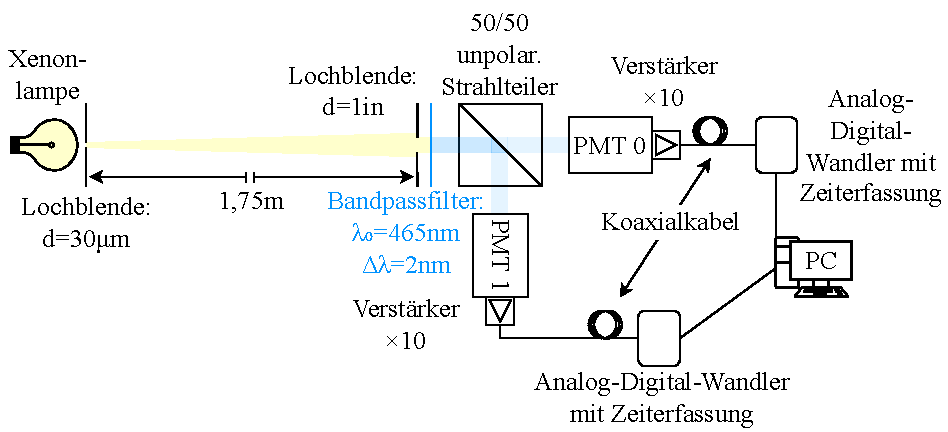
\includegraphics[width=0.9\linewidth]{images/Aufbau/Aufbau.pdf}
    \caption{Abgebildet ist eine vereinfachte Skizze des verwendeten Aufbaus, welche die konzeptuell wichtigsten Bauteile darstellt.}
    \label{fig:Versuchsaufbau}
\end{figure}
\todo{Fix Größe des Bildes, fontsize, abstand von pinhole hinzufügen}
Als Lichtquelle wird eine Xenon Lampe gewählt. 
Als Gasentladungslampe emittiert diese nach \autoref{ssec:Intensitäteninterferometrie} chaotisches Licht, welches bunching aufweist. 
Da nach dem van Cittert-Zernike Theorem der Winkeldurchmesser der Lichtquelle invers proportional zur Breite von $g^{(2)}(\bm{\rho})$ ist, ist weiterhin darauf zu achten die Ausdehnung der Lichtquelle einzuschränken, damit überhaupt korrelierte Photonen am Detektor vorliegen. 
Zu diesem Zweck ist eine kreisförmige Lochblende mit einem Durchmesser von $d=30\,\mathrm{\mu m}$ verbaut. 
Mit der Distanz $x=1,75\,\mathrm{m}$ zwischen Lichtquelle und dem restlichen Aufbau ergibt sich so ein Winkeldurchmesser von $\Delta \theta \approx \frac{d}{x} = 3,53\,\mathrm{asec}$. 
Es sei darauf hingewiesen, dass die größten Winkelsurchmesser von Sternen im Bereich von tausendstel Bogensekunden liegen \cite{hanburybrownAngularDiameters321974}, also etwa drei Größenordnungen kleiner sind, als der hier geschaffene \glqq künstliche Stern\grqq. \\
Um dem eintretenden Lichtstrahl eine definierte Breite zu geben, wird vor dieser zusätzlich durch eine Lochblende mit einem Durchmesser von einem Zoll geleitet. 
\todo{warum?}
Wie in \autoref{ssec:Michelson Sterninterferometer} beschrieben, ist für eine Messung der räumlichen Kohärenz auch eine nicht verschwindende Kohärenzzeit relevant. 
Da diese indirekt proportional zu spektralen Breite der Quelle ist, wird an dieser Stelle ein enger Bandpassfilter mit einer annähernd rechteckförmigen Transmissivität verbaut. 
Dieser hat nach Herstellerangaben eine zentrale Wellenlänge von $\lambda_0 = 465\,\mathrm{nm}$ und eine Breite von  $\Delta\lambda = 2\,\mathrm{nm}$ \cite{4652OD4Ultra}. 
Anschließend wird der Strahl durch einen nicht polarisierenden 50/50 Strahlteilerwürfel aufgeteilt und zum Nachweis der Photonen auf zwei Photomulitplier (PMTs) gelenkt. 
Direkt am Ausgang der Photomulitplier werden die Pulse mit einem Verstärker um den Faktor 10 verstärkt. 
Anschließend werden die Signale durch variable Kombinationen an Kabellänge und -modell zu Analog-Digital Wandlern (ADCs) geleitet, wo diese digitalisiert werden. 
Aufgrund des von Natur aus geringen Signals, werden alle analogen Signale durch geschirmte Koaxialkabel geleitet, um das Einkoppel von Störsignalen zu erschweren. 
Die Zeiterfassung der einzelnen ADC-Werte zur späteren Korrelation erfolgt durch Verwendung des White Rabbit Systems (vgl. z.B. \cite{lipinskiWhiteRabbitPTP2011}), welches direkt mit den ADCs verbunden ist. 
Abschließend werden die Daten am PC zur späteren Korrelation gespeichert. \\

Aufgrund des speziellen Aufbaus ergeben sich einige Änderungen bezüglich der im vorangegangenen Abschnitt eingeführten Theorie. 
Auf diese soll hier eingegangen werden. 
Wie erwähnt ist der Winkeldurchmesser der Quelle vergleichsweise groß. 
Nach \autoref{eq:erste nulstelle von g2(rho) für lochblende} wird für die Distanz zur ersten Nullstelle der $g^{(2)}$-Funktion lediglich $\rho_0\approx3,3\,\mathrm{cm}$ erwartet. 
Das heißt, dass am Beobachtungsort lediglich in einem Kreis mit Radius $\rho_0$ korrelierte Photonen auftreten. 
Aufgrund der physischen Größe der PMTs ist es daher nicht möglich, $g^{(2)}(\rho)$ für verschiedene $\rho$ zu messen. 
Stattdessen wird $g^{(2)}$ in einem Intervall $\rho\in[0,1]$ Zoll gemessen. 
Dieses entspricht den Abständen, die korrelierte Photonen durch die Lochblende am Eingang des Strahlteilers haben können. 
Es wird also erwartet, einen erniedrigten Wert für $g^{(2)}(\rho)$ und damit $\tau_c$ zu messen. 
Dies ist in \autoref{fig:räumliche koh simulation} verdeutlicht. 
Um herauszufinden, um welchen Faktor die gemessene Amplitude von der theoretischen maximalen Amplitude abweicht, wird eine Simulation durchgeführt, die sowohl den Wert von $g^{(2)}$ für jeden Photonenabstand als auch die Wahrscheinlichkeit für diesen berücksichtigt. 
Dieser Faktor beträgt bei gegebenem Aufbau $k_s=0,62$. 
\todo{Wie zitiere ich diese Simulationen?}
\begin{figure}[htbp]
    \centering
    \includegraphics{images/Aufbau/g2(rho).pdf}
    \caption{Dargestellt ist links die $g^{(2)}$-Funktion, abhängig von der Separation $\rho$. Rechts ist das Ergebnis der Simulation abgebildet. In blau ist $g^{(2)}$ für jeden Photonenabstand dargestellt (dies entspricht der Kurve im linken Graphen), während in orange die simulierte Wahrscheinlichkeitsverteilung ein Photoenpaar bei gegebenen Abstand anzutreffen aufgetragen ist. Durch Multiplikation der beiden Kurven erhält man den Faktor, um welchen die räumliche Kohärenz verringert ist. Dieser beträgt $k_s=0,62$. Links ist zudem eingezeichnet, welchem $\rho\prime$ eine Verringerung um ebendiesen Faktor entsprechen würde. }
    \label{fig:räumliche koh simulation}
\end{figure}
\todo{Verstehe ich es richtig, dass g2 um ks verringert wird? D.h. g2-1 liegt bei 2*ks -1 nicht bei ks???}
Über den theoretischen Verlauf der Korrelationsfunktion lässt sich durch $k_s$ auf einen effektiven Teleskopabstand $\rho\prime$ schließen, bei dem ein infinitesimal dünner Strahl den selben Verlust an räumlicher Kohärenz aufweist. 
Dies ist auch in \autoref{fig:räumliche koh simulation} veranschaulicht. \\
Aus voriger Überlegung ist nun bekannt $\tau_c^{meas} = k_s\cdot\tau_c^{th}$. 
Um $\tau_c^{th}$ zu bestimmen wird eine weitere Simulation verwendet. 
Diese berechnet aus dem vom Hersteller gegebenen Transmissionsprektrum des Filters über das Wiener-Khintchine Theore, d.h. eine Fouriertransformation die erwartete $g^{(1)}$-Funktion, welche anschließen über die Siegert-Relation in $g^{(2)}(\tau, \rho=0)$ umgerechnet wird. 
Daraus folgt dann für den vorliegenden Fall $\tau_c^{th} = \int g^{(2)}(\tau, \rho=0) -1 = 0,152\,\mathrm{ps}$. 
Abschließend ergibt sich also für die erwartete Kohärenzzeit bei dem verwendeten Aufbau:
\begin{equation}
    \tau_c^{meas} = 0,152\,\mathrm{ps}\cdot 0,62 = 94\,\mathrm{fs}
\end{equation}


